\documentclass[
10pt,
aspectratio=169,
]{beamer}


\usepackage{lipsum}
\usepackage{tikz}
\usepackage{circuitikz}
\usepackage{amssymb}
\usepackage{subcaption}
%\usepackage{subfig}

\title{TP Traitements Numériques Avancés}
\subtitle{Ecouteurs à réduction de bruit}
\date{Promo ESE 2022}
\author{Nicolas Guérin et Emma Perret}
%\institute{date}

\usetheme{ensea}  


\begin{document}

\begin{frame}
\titlepage
\end{frame}

%%% INTRODUCTION %%%
\section{Introduction}
\begin{frame} 
\frametitle{Introduction} 
Pour chaque bloc il faut réfléchir aux fréquences d'échantillonnage et de coupure mais également à la bande passante et au gain de cette bande. Il faut également penser à l'ordre du filtre. Pour chauqe signal, la fréquence d'échantillonnage et la longueur des mots sont déjà donnés.\\
Pour un signal PCM, nous pouvon facilement trouver la bande passante et le rapport signal à bruit :
\begin{enumerate} 
\item La bande passante équivaut à la fréquence d'échantillonnage ($f_e ~ ou ~ f_s$) divisée par deux.
\item Le rapport signal à bruit ($RSB ~ ou ~ SNR$) se définit de la sorte : $RSB = 6.02 * N + 1.76 $ avec $N ~ : ~ la ~ longueur ~ des ~ mots$. Il s'exprime en $dB$.
\item Pour un signal sur 16 bits, $RSB = 98 dB$.
\item Nous acceptons un $RSB - 4dB$. Pour cela, nous sommes obligés de passer par un dithering. Sans le dithering, le $RSB$ est de $-8 dB$ ce qui n'est pas acceptable.
\end{enumerate}
\end{frame}

\begin{frame} 
\frametitle{Introduction} 
Nous avons donc listé les données pour tous les signaux PCM.\\
Pour le signal de sortie de l'égalisateur : 
\begin{enumerate} 
\item $f_e = 48 kHz$
\item $Bande-passante = f_e/2 = 24 kHz$
\item $N = 20 bits$
\item $RSB = 122.16 dB$
\item $RSB_{accepte} = RSB - 4 = 118.16 dB$

\end{enumerate}
\vspace*{0.7cm}
Pour le signal de sortie du SR converter : 
\begin{enumerate} 
\item $f_e = 48 kHz$
\item $Bande-passante = f_e/2 = 24 kHz$
\item $N = 16 bits$
\item $RSB = 98.08 dB$
\item $RSB_{accepte} = RSB - 4 = 94.08 dB$

\end{enumerate}
\end{frame}

\begin{frame} 
\frametitle{Introduction} 
Pour le signal de sortie du player audio : 
\begin{enumerate} 
\item $f_e = 44.1 kHz$
\item $Bande-passante = f_e/2 = 22.05 kHz$
\item $N = 16 bits$
\item $RSB = 98.08 dB$
\item $RSB_{accepte} = RSB - 4 = 94.08 dB$

\end{enumerate}
\vspace*{0.7cm}
Pour les signaux de sortie du micro et du PDM modulator : 
\begin{enumerate} 
\item $f_e = 6.144 MHz$
\item $Bande-passante = f_e/2 = 3.72 MHz$
\item $N = 1 bits$
\item $RSB = 122.16 dB$
\item $RSB_{accepte} = RSB - 4 = 118.16 dB$

\end{enumerate}
\end{frame}
%%% FIN INTRODUCTION %%%

%%% PARTIE 1 : PDM %%%
\section{Partie 1 : PDM}
\subsection{Modulateur PDM}
\begin{frame} 
\frametitle{Partie 1 : Modulateur PDM} 
Le modulateur PDM permet de moduler un signal analogique en un signal binaire en fonction de la densité du signal. En effet, plus l'amplitude du signal analogique est élevée, plus le signal binaire sera constitué d'une suite longue de 1.\\
\vspace*{0.3cm}
La génération du modulteur PDM a déjà été faite. Après avoir compris son fonctionnement, nous sommes donc directement passés au démodulateur PDM.
\end{frame}

\subsection{Démodulateur PDM}
\subsubsection{Théorie}
\begin{frame} 
\frametitle{Partie 1 : Démodulateur PDM} 
\framesubtitle{Théorie} 
La fréquence d'échantillonnage d'entrée vaut $f_e=6.144 MHz$ et celle de la sortie vaut $f_e = 48 kHz$. Il y a un rapport de 128 entre les deux.\\
Il faut sous-échantillonner mais si nous échantillonnons par 128, cela est trop brutal et entraîne un ordre de filtre trop élevé et une pulsation de coupure très faible. Il faut donc faire par étape. \\
Mais avant de sous-échantilloner il faut filtrer. Nous avons choisi de prendre un filtre FIR, cela nous permet aussi de conserver la forme du signal puisque c'est un filtre à phase linéaire. Cependant le FIR entraîne des problèmes de latence car nous avons un RSB élevé ($120 dB$). Il faut donc faire attention au délai.
\end{frame}

\subsubsection{Signal d'entrée}
\begin{frame}
\frametitle{Partie 1 : Démodulateur PDM} 
\framesubtitle{Signal d'entrée} 
Nous observons d'abord le signal d'entrée~\ref{fig:entrée} : 
\begin{figure}[h]
    \centering
    \includegraphics[scale=0.2]{Images/entrée.png}
    \caption{Signal d'entrée}
\end{figure}
\end{frame}

\subsubsection{Mise en place des FIR}
\begin{frame} 
\frametitle{Partie 1 : Démodulateur PDM} 
\framesubtitle{FIR : Mise en place} 
Dans un premier temps nous décidons de sous-échantilloneur par 16 puis par 8 (le produit des deux donne bien 128). \\
Nous utilisons Filter Designer pour designer nos filtres FIR.\\
Pour le filtre avant le sous-échantillonneur par 16, nous prenons : 
\begin{enumerate}
    \item $f_s~=~6.144~MHz$
    \item $f_{stop}~=~f_e/16~=~384~kHz$
    \item $A_{stop}~=~120~dB$
\end{enumerate}
\vspace*{0.7cm}
Pour le filtre avant le sous-échantillonneur par 8, nous prenons : 
\begin{enumerate}
    \item $f_s~=~384~kHz$
    \item $f_{stop}~=~f_e/16~=~24~kHz$
    \item $A_{stop}~=~120~dB$
\end{enumerate}
\end{frame}

\begin{frame}
\frametitle{Partie 1 : Démodulateur PDM} 
\framesubtitle{FIR : Mise en place} 
Nous créons nos deux filtres : 
\begin{figure}[h]
    \centering
    \includegraphics[scale=0.2]{Images/FIR.png}
    \caption{Filtres FIR}
\end{figure}
\end{frame}

\begin{frame}
\frametitle{Partie 1 : Démodulateur PDM} 
\framesubtitle{FIR : Sous échantillonneur par 16}  
Nous observons les sorties de chaque sous-échantillonneur : 
\begin{figure}[h]
    \centering
    \includegraphics[scale=0.2]{Images/signal16.png}
    \caption{Sortie du sous-échantillonneur par 16}
\end{figure}
\end{frame}

\begin{frame}
\frametitle{Partie 1 : Démodulateur PDM} 
\framesubtitle{FIR : Sous échantillonneur par 8} 
Voici alors notre sortie finale du démodulateur PDM : 
\begin{figure}[h]
    \centering
    \includegraphics[scale=0.2]{Images/signal8.png}
    \caption{Sortie du sous-échantillonneur par 8}
\end{figure}
\end{frame}

\subsubsection{Améliorations}
\begin{frame}
\frametitle{Partie 1 : Démodulateur PDM} 
\framesubtitle{Améliorations} 
Nous pouvons améliorer le démodulateur PDM en faisant plus d'étapes. En effet, les ordres de nos filtres sont encore assez élevés et créent un certain délai.\\
Nous pouvons faire {8 puis 4 puis 4} ou encore {4 puis 4 puis 4 puis 2}.\\
Plus nous auront de blocs, plus la latence sera minimale.\\
\vspace{0.5cm}
Par ailleurs, la latence est aussi dûe au choix du filtre. En effet, un filtre FIR crée un certain délai.\\
Au lieu de créer plus de bloc, nous décidons de changer de filtre et d'opter pour des filtres IIR. Nous avons alors le choix entre un filtre Butterworth, Chebytchev type I, Chebytchev type II ou Elliptique.\\
Pour le choix du type de IIR, nous regarderons la phase et l'ordre.
\end{frame}

\subsubsection{Mise en place des IIR}
\begin{frame}
\frametitle{Partie 1 : Démodulateur PDM} 
\framesubtitle{IIR : Choix du type} 
Voici les phases des 4 filtres designés pour être placé avant le sous-échantillonneur par 16 : 
\begin{figure}
\centering
\begin{subfigure}{0.4\textwidth}
    \includegraphics[scale=0.3]{Images/Phase_IIR_butterworth.PNG}
    \caption{Butterworth}
\end{subfigure}
\hfill
\begin{subfigure}{0.4\textwidth}
    \includegraphics[scale=0.3]{Images/Phase_IIR_cheby_1.PNG}
    \caption{Chebytchev type I}
\end{subfigure}
\hfill
\begin{subfigure}{0.4\textwidth}
    \includegraphics[scale=0.3]{Images/Phase_IIR_cheby_2.PNG}
    \caption{Chebytchev type I}
\end{subfigure}
\begin{subfigure}{0.4\textwidth}
    \includegraphics[scale=0.3]{Images/Phase_IIR_elliptic.PNG}
    \caption{Elliptique}
\end{subfigure}
        
\caption{Phases des filtres IIR}
\label{fig:phases}
\end{figure}
\end{frame}

\begin{frame}
\frametitle{Partie 1 : Démodulateur PDM} 
\framesubtitle{IIR : Choix du type} 
Les filtres Butterworth a un retournement de phase ce que nous souhaitons évité. Le filtre de Chebytchev type I a une phase qui atteint une valeure minimale importante en valeur absolue.Nouos éliminons ces deux là.\\
La différence entre Chebytchev type II et Elliptique se fait au niveau de l'ordre. En effet le filtre de Chebytchev type II proposé par FilterDesigner est un ordre 104 alors que l'Elliptique est un ordre 22. Comme nous cherchons à minimiser l'ordre, nous choississons un filtre IIR elliptique.
\end{frame}

\begin{frame}
\frametitle{Partie 1 : Démodulateur PDM} 
\framesubtitle{IIR : Mise en place} 
Nous utilisons alors ces filtres : 
\begin{figure}[h]
    \centering
    \includegraphics[scale=0.2]{Images/IIR.png}
    \caption{Filtres FIR}
\end{figure}
\end{frame}

\begin{frame}
\frametitle{Partie 1 : Démodulateur PDM} 
\framesubtitle{IIR : Sous échantillonneur par 16}  
Nous observons les sorties de chaque sous-échantillonneur : 
\begin{figure}[h]
    \centering
    \includegraphics[scale=0.2]{Images/signal16_IIR.png}
    \caption{Sortie du sous-échantillonneur par 16}
\end{figure}
\end{frame}

\begin{frame}
\frametitle{Partie 1 : Démodulateur PDM} 
\framesubtitle{IIR : Sous échantillonneur par 8}  
Voici alors notre sortie finale du démodulateur PDM : 
\begin{figure}[h]
    \centering
    \includegraphics[scale=0.2]{Images/signal8_IIR.png}
    \caption{Sortie du sous-échantillonneur par 8}
\end{figure}
\end{frame}

\subsubsection{Comparaison FIR et IIR}
\begin{frame}
\frametitle{Partie 1 : Démodulateur PDM} 
\framesubtitle{Comparaison FIR et IIR}  
Nous constatons bien que les IIR suppriment la latence : 
\begin{figure}
\centering
\begin{subfigure}{0.4\textwidth}
    \includegraphics[scale=0.3]{Images/lat_FIR_16.PNG}
    \caption{Filtre FIR avant sous-échantillonneur 16}
\end{subfigure}
\hfill
\begin{subfigure}{0.4\textwidth}
    \includegraphics[scale=0.3]{Images/lat_FIR_8.PNG}
    \caption{Filtre FIR avant sous-échantillonneur 8}
\end{subfigure}
\hfill
\begin{subfigure}{0.4\textwidth}
    \includegraphics[scale=0.3]{Images/lat_IIR_16.PNG}
    \caption{Filtre IIR avant sous-échantillonneur 16}
\end{subfigure}
\begin{subfigure}{0.4\textwidth}
    \includegraphics[scale=0.3]{Images/lat_IIR_8.PNG}
    \caption{Filtre IIR avant sous-échantillonneur 8}
\end{subfigure}
        
\caption{Comparaison des latences}
\end{figure}
\end{frame}
%%% FIN PARTIE 1 %%%

%%% PARTIE 2 : SRC %%%
\section{Partie 2 : SRC}
\begin{frame} 
\frametitle{Partie 2 : Sample-Rate Converter} 
\framesubtitle{Démarche: } 
Nous allons créer un étage Sample Rate Converter :
\fbox{$F_{s_{in}}=44,1  kHz \quad F_{s_{out}}=48 kHz$ }
\begin{itemize}
\item[•] Rapport de réduction :$ \frac{480}{441}=\frac{160}{147}$ \textbf{Problème:} Pour sur et sous échantillonner de cet ordre de grandeur, la puissance de calcul demandée est considérable nous choisirons plutôt de décomposer cette fraction en facteur premier pour mettre des filtres plus petit en cascade.
\item[•]Décomposons en facteurs premier : $\frac{160}{147}=\frac{2}{3} \times \frac{4}{7} \times \frac{4}{7} \times 5$
\item[•]Nous allons générer nos filtres avec l'application matlab \textbf{filter designer} onglet Polyphase Sample-Rate
\end{itemize}
Voici un schéma de la cascade que nous allons implémenter; le premier bloc est généré par Filter Designer et les deux suivants sont réaliser grâce a une implémentation polyphase pour réussir à obtenir un rapport $\frac{L}{M}=\frac{4}{7}<1$ de ré-échantillonnage qui n'introduise pas de délai sur le filtrage.
\begin{figure}[h!]
\begin{flushleft}
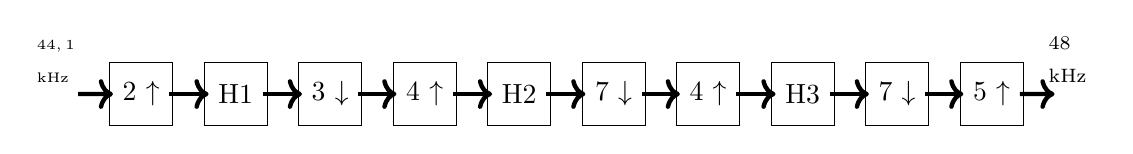
\begin{tikzpicture}[scale=0.4]
\draw (0,0) rectangle node (d71) { 2 $\uparrow$} (2,2);
\draw (3,0) rectangle node (H1){H1} (5,2);
\draw (6,0) rectangle node (41) {3 $\downarrow$}(8,2);
\draw (9,0) rectangle node (d72) {4 $\uparrow$}(11,2);
\draw (12,0) rectangle node (H2) {H2 }(14,2);
\draw (15,0) rectangle node (42) {7 $\downarrow$}(17,2);
\draw (18,0) rectangle node (3) {4 $\uparrow$} (20,2);
\draw (21,0) rectangle node (H3){H3} (23,2);
\draw (24,0) rectangle node (2) {7 $\downarrow$}(26,2);
\draw (27,0) rectangle node (5) {5 $\uparrow$} (29,2);
%Drawing arrows
\draw [->, ultra thick] (-1,1) -- node[above left,text width=0.6cm]{ {\tiny  $44,1$ kHz}}(d71.west);
\draw [->, ultra thick] (d71.east) -- (H1.west);
\draw [->, ultra thick] (H1.east) -- (41.west);
\draw [->, ultra thick] (41.east) -- (d72.west);
\draw [->, ultra thick] (d72.east) -- (H2.west);
\draw [->, ultra thick] (H2.east) -- (42.west);
\draw [->, ultra thick] (42.east) -- (3.west);
\draw [->, ultra thick] (3.east) -- (H3.west);
\draw [->, ultra thick] (H3.east) -- (2.west);
\draw [->, ultra thick] (2.east) -- (5.west);
\draw [->, ultra thick] (5.east) -- node[above right,text width=0.6cm]{{\scriptsize  $48$ kHz}} (30,1);
\end{tikzpicture}
\end{flushleft}
\end{figure}


\end{frame}
\begin{frame}
\frametitle{Génération Premier étage de la cascade}
\framesubtitle{}
\begin{figure}[!h]
\center
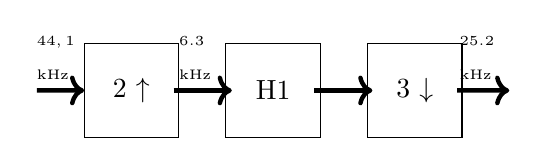
\begin{tikzpicture}[scale=0.6]
\draw (0,0) rectangle node (d71) {2 $\uparrow$} (2,2);
\draw (3,0) rectangle node (H1){H1} (5,2);
\draw (6,0) rectangle node (41) {3 $\downarrow$}(8,2);

\draw [->, ultra thick] (-1,1) -- node[above ,text width=0.6cm]{ {\tiny  $44,1$ kHz}}($(d71.west)+(-0.4,0)$);
\draw [->, ultra thick]($ (d71.east)+(0.3,0)$) -- node [above ,text width=0.6cm]{{\tiny $6.3$ kHz}} ($(H1.west)+(-0.3,0)$);
\draw [->, ultra thick] ($(H1.east)+(0.3,0)$) -- ($(41.west)+(-0.3,0)$);
\draw [->, ultra thick] ($(41.east)+(0.3,0)$) -- node [above ,text width=0.6cm]{{\tiny $25.2$ kHz}} (9,1);
\end{tikzpicture}
\caption{Représentation des blocs qui réalisent le premier étage}
\end{figure}
Nous avons choisi cet étage en première position car il permet de filtrer sans perdre d'informations sans pour autant trop augmenter la puissance de calcul due à l'upsampling.
\begin{figure}[!h]
\center
\includegraphics[scale=0.2]{Images/stage1.PNG} 
\caption{En haut: signal d'entrée sous-échantilloné, en bas: signal de  sortie du premier étage de la cascade de filtre}
\end{figure}

\end{frame}
\begin{frame}
\frametitle{Génération second étage de la cascade}
\framesubtitle{}
\begin{figure}[!h]
\center
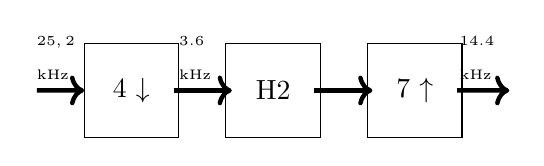
\begin{tikzpicture}[scale=0.6]
\draw (0,0) rectangle node (d71) {4 $\downarrow$} (2,2);
\draw (3,0) rectangle node (H1){H2} (5,2);
\draw (6,0) rectangle node (41) {7 $\uparrow$}(8,2);

\draw [->, ultra thick] (-1,1) -- node[above ,text width=0.6cm]{ {\tiny  $25,2$ kHz}}($(d71.west)+(-0.4,0)$);
\draw [->, ultra thick]($ (d71.east)+(0.3,0)$) -- node [above ,text width=0.6cm]{{\tiny $3.6$ kHz}} ($(H1.west)+(-0.3,0)$);
\draw [->, ultra thick] ($(H1.east)+(0.3,0)$) -- ($(41.west)+(-0.3,0)$);
\draw [->, ultra thick] ($(41.east)+(0.3,0)$) -- node [above ,text width=0.6cm]{{\tiny $14.4$ kHz}} (9,1);
\end{tikzpicture}
\caption{Représentation des blocs qui réalisent le premier étage}
\end{figure}
Le filtre polyphase est construit de la manière suivante : On réalise une répartition dans 4 branches des composants du vecteur colonne obtenu en sortie de l'étage précédent. On introduit  7 sous-branche déterminées à partir de la branche de plus haut niveau. sur chacune de ces sous branches on filtre par un second ordre. Ce second ordre est issue de la décomposition d'un filtre général en plusieurs niveaux par branches et sous-branches. Ainsi pour la branche 3, sous branche 6 on aura un filtre $H_{3,6}$ du second degré issue du filtre général $H$. On reproduit ce schéma pour le dernier étage également. 

%\begin{figure}[!h]
%\center
%\includegraphics[scale=0.2]{Images/stage2.PNG} 
%\caption{En haut: signal d'entrée deuxième étage, en bas: signal de  sortie du second étage de la cascade de filtre}
%\end{figure}

\end{frame}
\begin{frame}
\frametitle{Génération dernier étage de la cascade}
\framesubtitle{}
\begin{figure}[!h]
\center
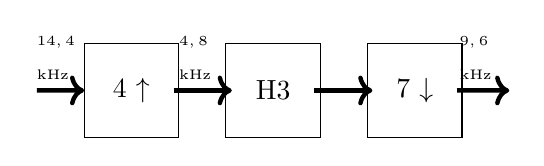
\begin{tikzpicture}[scale=0.6]
\draw (0,0) rectangle node (d71) {4 $\uparrow$} (2,2);
\draw (3,0) rectangle node (H1){H3} (5,2);
\draw (6,0) rectangle node (41) {7 $\downarrow$}(8,2);

\draw [->, ultra thick] (-1,1) -- node[above ,text width=0.6cm]{ {\tiny  $14,4$ kHz}}($(d71.west)+(-0.4,0)$);
\draw [->, ultra thick]($ (d71.east)+(0.3,0)$) -- node [above ,text width=0.6cm]{{\tiny $4,8$ kHz}} ($(H1.west)+(-0.3,0)$);
\draw [->, ultra thick] ($(H1.east)+(0.3,0)$) -- ($(41.west)+(-0.3,0)$);
\draw [->, ultra thick] ($(41.east)+(0.3,0)$) -- node [above ,text width=0.6cm]{{\tiny $9,6$ kHz}} (9,1);
\end{tikzpicture}
\caption{Représentation des blocs qui réalisent le dernier étage}
\end{figure}

%\begin{figure}[!h]
%\center
%\includegraphics[scale=0.2]{Images/stage3.PNG} 
%\caption{En haut: signal d'entrée sous-échantilloné, en bas: signal de  sortie du premier étage de la cascade de filtre}
%\end{figure}

\end{frame}
\begin{frame}
\frametitle{Upsampling de sortie}
\framesubtitle{}
\begin{figure}[!h]
\center
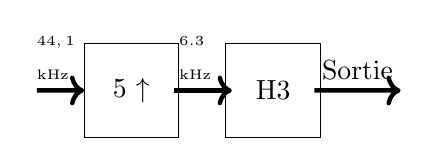
\begin{tikzpicture}[scale=0.6]
\draw (0,0) rectangle node (d71) {5  $\uparrow$} (2,2);
\draw (3,0) rectangle node (H1){H3} (5,2);


\draw [->, ultra thick] (-1,1) -- node[above ,text width=0.6cm]{ {\tiny  $44,1$ kHz}}($(d71.west)+(-0.4,0)$);
\draw [->, ultra thick]($ (d71.east)+(0.3,0)$) -- node [above ,text width=0.6cm]{{\tiny $6.3$ kHz}} ($(H1.west)+(-0.3,0)$);
\draw [->, ultra thick] ($(H1.east)+(0.3,0)$) -- node [above] {Sortie} ($(7,1)+(-0.3,0)$);

\end{tikzpicture}
\caption{Représentation des blocs qui réalisent le premier étage}
\end{figure}

\begin{figure}[!h]
\center
\includegraphics[scale=0.3]{Images/output_poly.PNG} 
\caption{Signal PCM à 48 kHz}
\end{figure}
\end{frame}

\begin{frame}
\frametitle{Addition des signaux}
Nous effectuons la somme des signaux et le rééquilibrage des tailles pour les vecteurs.
\end{frame}
%%% FIN PARTIE 2 %%%
%%%Début partie trois %%

\begin{frame}
\frametitle{Méthode fréquentielle}
On applique l'algorithme WOLA pour permettre la reconstruction parfaite du signal. 
\begin{enumerate}
\item On débute par sélectionner une fenêtre (Hamming) et un taux de recouvrement (50\%) et vérifier le critère COLA par la fonction \texttt{iscola}.
\item On génère deux vecteurs avec une répétition de ces fenêtres et un décalage de 50\% entre les deux vecteurs.
\item On applique les vecteurs au signal et on 
\end{enumerate}
\end{frame}

%%% PARTIE 3 : Regulateur %%%
%% TEMPOREL%%

\section{Parie 3 : Banc de filtres}
\subsection{Reconstruction du signal - Méthode fréquentielle}
\begin{frame}
\frametitle{Méthode fréquentielle}
On applique l'algorithme WOLA pour permettre la reconstruction parfaite du signal. 
\begin{enumerate}
\item On débute par sélectionner une fenêtre (Hamming) et un taux de recouvrement (50\%) et vérifier le critère COLA par la fonction \texttt{iscola}.
\item On génère deux vecteurs avec une répétition de ces fenêtre et un décalage de 50\%entre les deux vecteurs.
\item On applique les vecteurs au signal et on 
\end{enumerate}
\end{frame}

\subsection{Méthode temporelle}

\begin{frame}
\frametitle{Partie 3 : Banc de filtres temporels} 
\framesubtitle{Principe}
Dans un premier temps nous allons utiliser une méthode temporelle et faire un banc de filtres octaves à 9 étages pour avoir 10 bandes comme souhaité. \\
Le but est d'ajouter un gain par bande entre l'analyse et la synthèse pour créer l'égaliseur. \\
Nous construisons 4 filtres complémentaires avec la fonction $firpr2chfb$ pour ce banc de filtres. \\ 
Le vu mètre correspond simplement à la mesure de l'énergie sur chaque bande et sera matérialisé par une matrice.
\end{frame}

\begin{frame}
\frametitle{Partie 3 : Banc de filtres temporels} 
\framesubtitle{Analyse}
Pour l'analyse, nous utilisons les filtres $H_0$ et $H_1$ et nous sous-échantillonnons par 2 à chaque étage comme ci-dessous.
\begin{figure}
 \centering
\includegraphics[width=10cm]{Images/analyse.png}
 \caption{Analyse du banc de filtres}
\end{figure}
\end{frame}



%\begin{frame}
%\frametitle{Upsampling de sortie}
%\framesubtitle{}
%\begin{figure}[!h]
%\center
%\begin{tikzpicture}[scale=0.6]
%\draw (0,0) rectangle node (d71) {5  $\uparrow$} (2,2);
%\draw (3,0) rectangle node (H1){H3} (5,2);
%
%
%\draw [->, ultra thick] (-1,1) -- node[above ,text width=0.6cm]{ {\tiny  $44,1$ kHz}}($(d71.west)+(-0.4,0)$);
%\draw [->, ultra thick]($ (d71.east)+(0.3,0)$) -- node [above ,text width=0.6cm]{{\tiny $6.3$ kHz}} ($(H1.west)+(-0.3,0)$);
%\draw [->, ultra thick] ($(H1.east)+(0.3,0)$) -- node [above] {Sortie} ($(7,1)+(-0.3,0)$);
%
%\end{tikzpicture}
%\caption{Représentation des blocs qui réalisent le premier étage}
%\end{figure}

%\begin{figure}[!h]
%\center
%\includegraphics[scale=0.3]{Images/output_poly.PNG} 
%\caption{Signal PCM à 48 kHz}
%
%\end{figure}
%\end{frame}

\begin{frame}
\frametitle{Partie 3 : Banc de filtres temporels} 
\framesubtitle{Traitement : gains}
Pour la partie traitement entre l'analyse et la synthèse, il s'agit juste d'offrir la possbilité d'appliquer à chaque bande le gain souhaité pour modifier l'ambiance de l'audio. Il suffit donc de multiplier chacun des 10 signaux de sortie de l'analyse par un gain associé (exmple : nous multiplions $x_1$ par $G_1$ etc.).
\end{frame}

\begin{frame}
\frametitle{Partie 3 : Banc de filtres temporels} 
\framesubtitle{Synthèse}
Pour l'analyse, nous utilisons les filtres $F_0$ et $F_1$ et nous sur-échantillonnons par 2 à chaque étage comme ci-dessous.
\begin{figure}
    \centering
    \includegraphics[width=12cm]{Images/synthèse.png}
    \caption{Synthèse du banc de filtres}
\end{figure}
\end{frame}



\end{document}
